% ALGUNOS PAQUETES REQUERIDOS (EN UBUNTU): %
% ========================================
% %
% texlive-latex-base %
% texlive-latex-recommended %
% texlive-fonts-recommended %
% texlive-latex-extra %
% texlive-science %
% texlive-lang-spanish (en ubuntu 13.10) %
% ******************************************************** %

\documentclass[a4paper]{article}
\usepackage[spanish, es-nodecimaldot]{babel}
\usepackage[utf8]{inputenc}
\usepackage{fancyhdr}
\usepackage[pdftex]{graphicx}
\usepackage{sidecap}
\usepackage{caption}
\usepackage{subcaption}
\usepackage{booktabs}
\usepackage{makeidx}
\usepackage{float}
\usepackage{amsmath, amsthm, amssymb}
\usepackage{amsfonts}
\usepackage{sectsty}
\usepackage{wrapfig}
\usepackage{listings}
\usepackage{pgfplots}
\usepackage{pgfplotstable}
\usepackage{enumitem}
\usepackage[hidelinks]{hyperref}
\usepackage{listings}
\usepackage{listingsutf8}

\linespread{factor}

\definecolor{mygreen}{rgb}{0,0.6,0}
\definecolor{mygray}{rgb}{0.5,0.5,0.5}
\pgfplotsset{compat=1.8}
\setlist[enumerate]{label*=\arabic*.}
\lstset{
	inputencoding=utf8/latin1,
	language=C++,
	basicstyle=\ttfamily,
	keywordstyle=\bfseries\color{blue},
	stringstyle=\color{red}\ttfamily,
	commentstyle=\color{mygreen}\ttfamily,
	morecomment=[l][\color{magenta}]{\#},
	numbers=left,
	numberstyle=\color{mygray}
}

\usepackage{fancyhdr}
\pagestyle{fancy}
\fancyhf{}
\fancyhead[LO]{Problemas, Algoritmos y Programación}
\fancyhead[RO]{Trabajo Práctico N\textsuperscript{o} 1}
%\fancyfoot[LO]{\small{Shai Bianchi, Martín Jedwabny, Manuel Mena, Iván Pondal}}
\fancyfoot[RO]{\thepage}
\renewcommand{\headrulewidth}{0.5pt}
\renewcommand{\footrulewidth}{0.5pt}
\setlength{\textwidth}{16cm}
\setlength{\hoffset}{-1.1cm}
\setlength{\headsep}{0.5cm}
\setlength{\textheight}{25cm}
\setlength{\voffset}{-1.75cm}
\setlength{\headwidth}{\textwidth}
\setlength{\headheight}{13.1pt}
\renewcommand{\baselinestretch}{1.1} % line spacing

\usepackage{caratula}

\allowdisplaybreaks
\newcommand{\ord}{\ensuremath{\operatorname{O}}}
\newcommand{\nat}{\ensuremath{\mathbb{N}}}
\newcommand{\real}{\ensuremath{\mathbb{R}}}
\newcommand{\acr}[1]{\lowercase{\textsc{#1}}}
\newcommand{\comp}{\ensuremath{^{\operatorname{C}}}}
\newcommand{\argmax}{\operatornamewithlimits{arg\,m\acute{a}x}}

\newcommand{\subheading}[1]{\vspace{1em} \noindent\textbf{#1} \nopagebreak
\smallskip \nopagebreak}

% Lemas, definiciones, etc.
\theoremstyle{plain}
  \newtheorem{prop}{Proposición}
  \newtheorem{lema}{Lema}
\theoremstyle{remark}
  \newtheorem{obs}{Observación}
\theoremstyle{definition}
  \newtheorem{defi}{Definición}

% Pseudocódigo
\usepackage[onelanguage, spanish]{algorithm2e}
    % \NoCaptionOfAlgo
    \LinesNumbered\RestyleAlgo{ruled}\IncMargin{1em}\DontPrintSemicolon
    \SetArgSty{}\SetCommentSty{textsf}\SetFuncSty{textsf}
    \SetKwInput{Input}{Entrada}
    \SetKwInput{Output}{Salida}
    \SetKwProg{For}{para}{ hacer}{fin}
    \SetKwProg{Fn}{función}{:}{fin}

\begin{document}
\materia{Introducción a la Robótica Móvil}
\submateria{Segundo cuatrimestre de 2016}
\titulo{Trabajo Práctico N\textsuperscript{o} 3}
\subtitulo{Localización basada en EKF: Predicción y corrección}
\integrante{Luis García Gómez}{675/13}{garcia\_luis\_94@hotmail.com}
\integrante{Manuel Mena}{313/14}{manuelmena1993@gmail.com}

\maketitle
% no footer on the first page
\thispagestyle{empty}
\newpage
\section{Ejecución de comandos y explicación de proceso}

\subsection{¿Qué empieza a suceder con la covarianza? ¿A qué se debe esto?. Dar una captura de pantalla y explicar lo observado.}

Previo a ejecutar los comandos pedidos en el enunciado del trabajo, la covarianza se presenta circular con centro en el robot. Luego de ejecutar los comandos pedidos, la covarianza empieza a cambiar de forma hasta llegar a ser una elipse con el eje mayor perpendicular al poste que se tiene en frente:

Sean 'x' e 'y' los ejes del robot, con 'y' paralelo a las ruedas del mismo (modelo diferencial), queda determinada una covarianza con forma de elipse cuyo eje mayor y menor son el eje 'y' y 'x' respectivamente. Esto puede explicarse a modo básico de la siguiente manera: La covarianza representa una región en la que su centro tiene probabilidad máxima de tener el poste a su frente. Esta probabilidad disminuye a medida que se analiza la mencionada región hacia sus extremos. Al momento de generar la covarianza, el filtro de Kalman, realiza estimaciones que determinan que sobre el eje 'y' la proporción en la que se puede mover el robot para que la probabilidad de tener el poste en frente sea significativa es mayor, no así en el eje 'x', determinando de esta manera los ejes mayor y menor mencionados al inicio.


A continuación se muestra una imagen del estado del robot una vez realizadas las instrucciones en RVIZ
\begin{center}
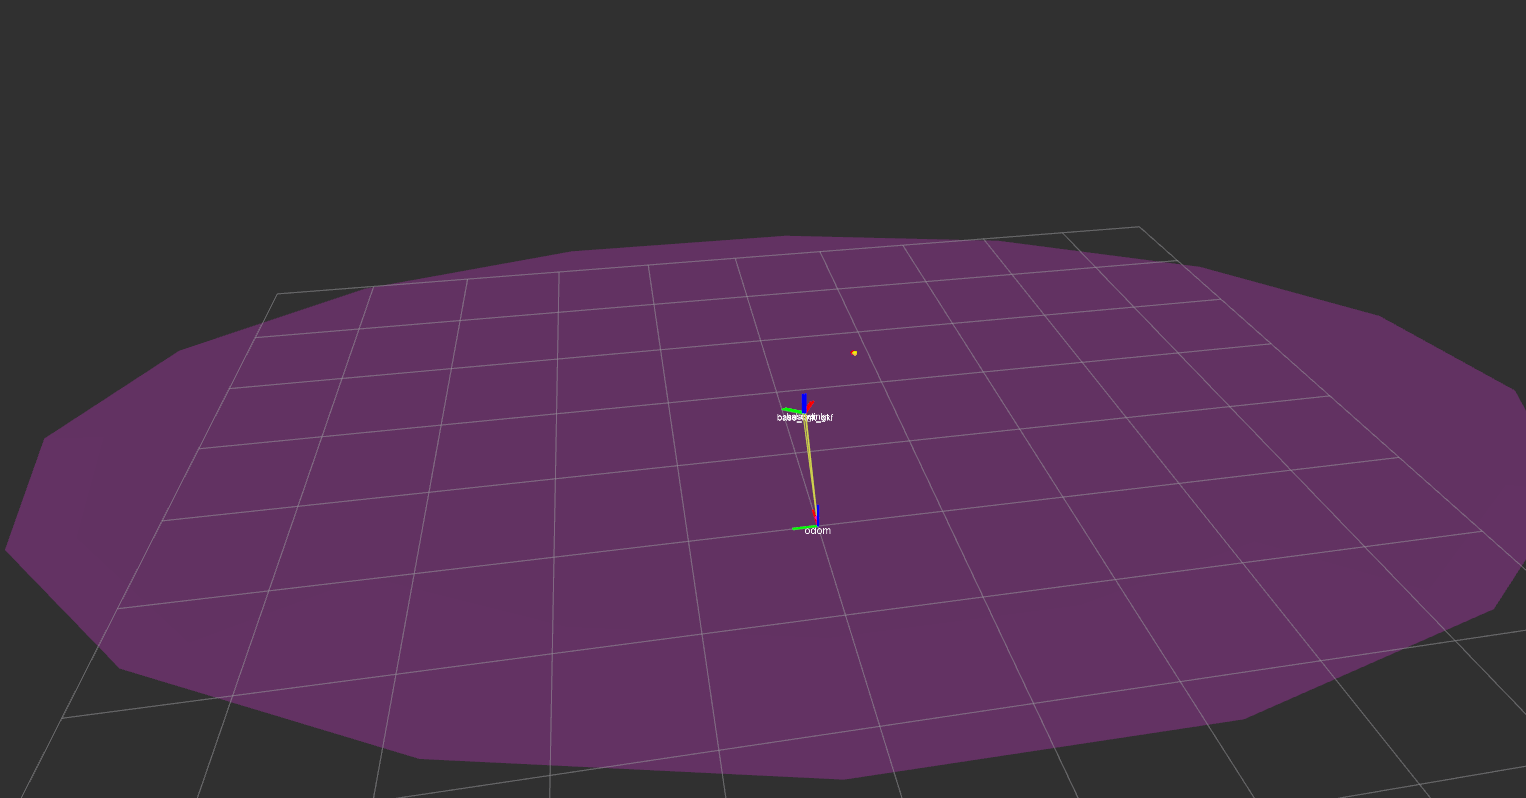
\includegraphics[scale=0.4]{tp3_ej1.png}
\end{center}
\section{Filtro de Kalman extendido para un robot omnidireccional}

\subsection*{Modelo de estado}

Para el modelo de estado $\vec{x}$ se usará el mismo que para el robot diferencial, $\vec{x} = (x, y, \theta)$. Por ser omnidireccional podría ahorrarse modelar la rotación de la posición, pero para ello debería asegurarse que el sistema de sensado, en este caso el laser, mantiene la misma rotación con la que comenzó.

\subsection*{Entradas de control}

En cuanto a las entradas de control $\vec{u}$ sí serán diferentes a la del robot diferencial, debido a que este puede moverse en línea recta hasta su objetivo, sin necesidad de hacer curvas. El modelo para ello es $\vec{u} = (V_x, V_y, V_{\theta})$. Es importante notar que la información de la velocidad es respecto a los ejes del mundo, no de los del robot.

\subsection*{Ruido del sensor}

El ruido del sensor se modelará con una variable aleatoria Normal de media 0 y varianza $Q$, donde $Q$ estará determinada por el fabricante de los actuadores.

\subsection*{Modelo de movimiento}

El modelo de movimiento será $f(\vec{x}, \vec{u}, \vec{w}) = (\vec{x} + V_x \times \Delta t + w_1, \vec{y} + V_y \times \Delta t + w_2, \vec{\theta} + V_{\theta} \times \Delta t + w_3)$.

El prior belief estará dado por $\hat{x}_t = f(\hat{x}_{t - 1}, \vec{u}_{t - 1}, \vec{0})$.

Para el modelo de movimiento, ambos Jacobianos serán matrices de identidad en $\real^{3 \times 3}$. Esto tiene mucho sentido en cuanto al Jacobiano de $f$ respecto a $\vec{x}$ ya que por ser omnidireccional puede moverse en cada eje independientemente del resto.

\subsection*{Mediciones}

Las mediciones al igual que con el robot diferencial tendrán dos componentes: el ángulo con respecto al robot, y la distancia hacia él. $\vec{z} = (\rho, \phi)$

\subsection*{Modelo de sensado}

Para cada landmark se tendrá una predicción de cómo debería verse segun una posición y un ruido. Esta prediccíon estará dada por $z^l = h^l(\vec{x}, \vec{v})$. Lo que devolverá $h$ será la distancia del landmark al robot sumado a un ruido y el ángulo del landmark respecto al robot sumado a un ruido.

$h^l(\vec{x}, \vec{v}) = (\sqrt{x_l^2 + y_l^2} + v_1, norm(atan2(y_l, x_l)) + v_2)$.

El Jacobiano de $h$ respecto a $\vec{x}$ es $H = \left(
\begin{matrix}
\frac{x}{\sqrt{x^2 + y^2}} & \frac{y}{\sqrt{x^2 + y^2}} \\
\frac{y}{x^2 + y^2} & \frac{-y}{x^2 + y^2} \\
\end{matrix}
\right)$

El Jacobiano de $h$ respecto a $\vec{v}$ es $V = \left(
\begin{matrix}
1 & 0 \\
0 & 1 \\
\end{matrix}
\right)$

Este modelo permanece igual al del robot diferencial.

\end{document}
